\documentclass[tikz,border=10pt]{standalone}
\usepackage{tikz}
\usetikzlibrary{patterns, arrows.meta, positioning, calc, decorations.pathmorphing}

\begin{document}
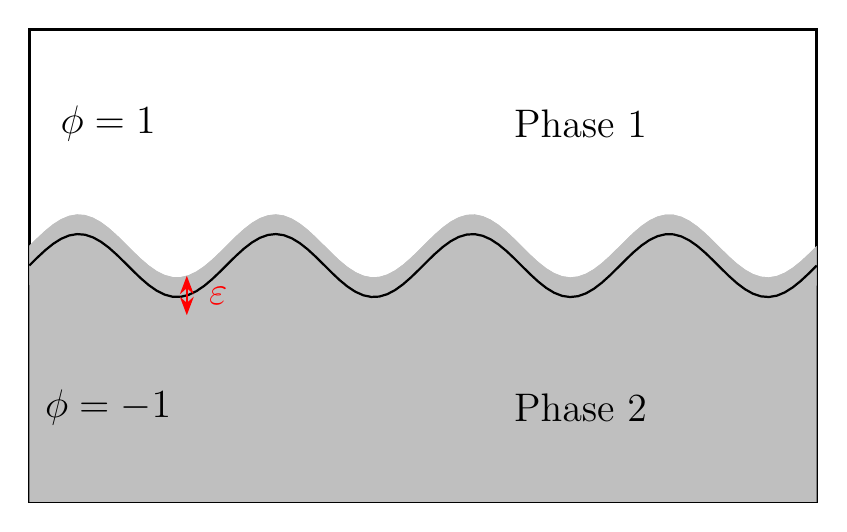
\begin{tikzpicture}
    % --- Style Definitions ---
    \tikzset{
        box style/.style={
            draw=black,
            very thick
        },
        interface style/.style={
            draw=black,
            thick
        },
        shaded region/.style={
            fill=gray!50
        },
        label text/.style={
            font=\Large,
            color=black
        },
        epsilon arrow/.style={
            <->,
            >=Stealth,
            thick,
            red
        }
    }

    % Box dimensions
    \def\boxwidth{10}
    \def\boxheight{6}

    % Wave parameters (derived from visual analysis)
    \def\amplitude{0.4}
    \def\wavelength{2.5}
    \def\yoffset{3}  % middle of box
    \def\epsilon{0.5} % interface width

    % --- 1. Draw the outer box ---
    \draw[box style] (0,0) rectangle (\boxwidth,\boxheight);

    % --- 2. Draw the gray shaded region ---
    % Upper boundary of shaded region
    \draw[shaded region, draw=none]
        plot[domain=0:\boxwidth, samples=100]
        (\x, {\yoffset + \amplitude*sin(360*\x/\wavelength) + \epsilon/2})
        -- (\boxwidth, 0) -- (0, 0) -- cycle;

    % Fill the entire shaded region properly
    \fill[gray!50]
        plot[domain=0:\boxwidth, samples=100]
        (\x, {\yoffset + \amplitude*sin(360*\x/\wavelength) + \epsilon/2})
        -- (\boxwidth, {\yoffset - \amplitude*sin(360*\boxwidth/\wavelength) - \epsilon/2})
        -- plot[domain=\boxwidth:0, samples=100]
        (\x, {\yoffset + \amplitude*sin(360*\x/\wavelength) - \epsilon/2})
        -- cycle;

    % --- 3. Draw the black wavy boundary (center line) ---
    \draw[interface style]
        plot[domain=0:\boxwidth, samples=100]
        (\x, {\yoffset + \amplitude*sin(360*\x/\wavelength)});

    % --- 4. Add phase labels ---
    \node[label text] at (1, 4.8) {$\phi = 1$};
    \node[label text] at (7, 4.8) {Phase 1};

    \node[label text] at (1, 1.2) {$\phi = -1$};
    \node[label text] at (7, 1.2) {Phase 2};

    % --- 5. Add epsilon arrow and label ---
    % Place at x=2 where we can see the interface clearly
    \def\arrowx{2}
    \pgfmathsetmacro{\arrowy}{\yoffset + \amplitude*sin(360*\arrowx/\wavelength)}

    \draw[epsilon arrow]
        (\arrowx, \arrowy - \epsilon/2) -- (\arrowx, \arrowy + \epsilon/2);

    \node[color=red, font=\Large] at (\arrowx + 0.4, \arrowy) {$\varepsilon$};

\end{tikzpicture}
\end{document}
